
\de{ĐỀ THI HỌC KỲ II NĂM HỌC 2022-2023}{THPT Nguyễn Trường Tộ - Huế}
\begin{center}
	\textbf{PHẦN 1 - TRẮC NGHIỆM}
\end{center}
\Opensolutionfile{ans}[ans/ans]
\begin{ex}%[0X2Y2-8]%[Dự án Đề kiểm tra HKII NH22-23-TinDatTran]%[THPT Nguyễn Trường Tộ - Huế]
Cho các số nguyên dương $k, n(0<k \leq n)$. Mệnh đề nào sau đây đúng?
\choice
{\True $\mathrm{C}_n^k=\dfrac{n !}{k !(n-k) !}$}
{$\mathrm{C}_n^k=\dfrac{n !}{(n-k) !}$}
{$\mathrm{C}_n^k=k!$}
{$\mathrm{C}_n^k=n!$}
\loigiai{
Ta có $\mathrm{C}_n^k=\dfrac{n!}{k!(n-k)!}$.
}
\end{ex}
\begin{ex}%[0D4Y4-2]%[Dự án Đề kiểm tra HKII NH22-23-TinDatTran]%[THPT Nguyễn Trường Tộ - Huế]
Cho tam thức $f(x)=a x^2+b x+c(a \neq 0)$, $\Delta=b^2-4 a c$. Ta có $f(x)>0, \forall x \in \mathbb{R}$ khi và chỉ khi:
\choice
{\True $\heva{&a>0 \\ &\Delta<0}$}
{$\heva{&a \geq 0 \\& \Delta<0}$}
{$\heva{&a>0 \\& \Delta \leq 0}$}
{$\heva{&a>0 \\& \Delta \geq 0}$}
\loigiai{
$f(x)>0, \forall x \in \mathbb{R}$ khi và chỉ khi $\heva{&a>0 \\&\Delta<0}$.
}
\end{ex}
\begin{ex}%[0H4Y2-1]%[Dự án Đề kiểm tra HKII NH22-23-TinDatTran]%[THPT Nguyễn Trường Tộ - Huế]
Xác định tâm $I$ và bán kính $R$ của đường tròn có phương trình $x^2+y^2-2 x+4 y+1=0$
\choice
{\True $I(1 ;-2)$, $R =2$}
{$I(1 ;-2)$, $R =1$}
{$I(-1 ; 2)$, $R=1$}
{$I(2 ;-4)$, $R =2$}
\loigiai{
Ta có $a=1$; $b=-2$; $c=1$.\\
Tâm và bán kính của đường tròn đã cho là $I(1;-2)$, $R=\sqrt{1^2+(-2)^2-1}=2$.
}
\end{ex}
\begin{ex}%[0H4Y1-1]%[Dự án Đề kiểm tra HKII NH22-23-TinDatTran]%[THPT Nguyễn Trường Tộ - Huế]
Trong mặt phẳng $O x y$, một vectơ pháp tuyến của đường thẳng $d\colon2 x-3 y+9=0$ là
\choice
{$\vec{n}=(3 ;-2)$}
{$\vec{n}=(-2 ;-3)$}
{$\vec{n}=(2 ; 3)$}
{\True $\vec{n}=(2 ;-3)$}
\loigiai{
Vectơ pháp tuyến của đường thẳng $d\colon2 x-3 y+9=0$ là $\vec{n}=(2;-3)$.
}
\end{ex}
\begin{ex}%[0X2B3-3]%[Dự án Đề kiểm tra HKII NH22-23-TinDatTran]%[THPT Nguyễn Trường Tộ - Huế]
Trong khai triển theo công thức nhị thức Newton của $(1+2 x)^5$ có bao nhiêu số hạng?
\choice
{$4$}
{\True $6$}
{$5$}
{$7$}
\loigiai{
Trong khai triển công thức nhị thức Newton của $(1+2x)^5$ có $6$ số hạng.
}
\end{ex}
\begin{ex}%[0H4B1-2]%[Dự án Đề kiểm tra HKII NH22-23-TinDatTran]%[THPT Nguyễn Trường Tộ - Huế]
Phương trình tham số của đường thẳng đi qua 2 điểm $A(3 ;-1)$ và $B(1 ; 5)$ là
\choice
{\True $\heva{&x=3+t \\ &y=-1-3 t}$}
{$\heva{&x=3-t \\ &y=-1-3 t}$}
{$\heva{&x=3+t \\ &y=-1+3 t}$}
{$\heva{&x=1-t \\ &y=5-3 t}$}
\loigiai{
Ta có $\overrightarrow{AB}=(-2;6)$. Véctơ chỉ phương của đường thẳng $AB$ là $\vec{u}=\dfrac{-1}{2}\overrightarrow{AB}=(1;-3)$.\\
Phương trình tham số của đường thằng $d$ là 
\[d\colon \heva{&x=3+t \\ &y=-1-3 t.}\]
}
\end{ex}
\begin{ex}%[0X2B3-3]%[Dự án Đề kiểm tra HKII NH22-23-TinDatTran]%[THPT Nguyễn Trường Tộ - Huế]
Hệ số của $x^5$ trong khai triển biểu thức $P=(2-3 x)^5$ bằng
\choice
{$357$}
{$628$}
{\True $-243$}
{$243$}
\loigiai{
Hệ số của $x^5$ trong khai triển biểu thức $P$ là $\mathrm{C}_5^5\cdot (-3)^5=-243$.
}
\end{ex}
\begin{ex}%[0D4B3-1]%[Dự án Đề kiểm tra HKII NH22-23-TinDatTran]%[THPT Nguyễn Trường Tộ - Huế]
Tập nghiệm của phương trình $\sqrt{x^2+x+1}=\sqrt{5+x}$ là
\choice
{$S=\{2\}$}
{$S=\varnothing$}
{$S=\{-2\}$}
{\True $S=\{2 ;-2\}$}
\loigiai{
\begin{align*}
&\sqrt{x^2+x+1}=\sqrt{5+x}\\
\Rightarrow &x^2+x+1=5+x\\
\Rightarrow &x^2-4=0\\
\Rightarrow &\hoac{&x=2\\&x=-2.}
\end{align*}
Thử lại, phương trình đã cho có hai nghiệm là $x=2$ và $x=-2$.\\
Vậy tập nghiệm của phương trình đã cho là $S=\{2;-2\}$.
}
\end{ex}
\begin{ex}%[0X3Y1-2]%[Dự án Đề kiểm tra HKII NH22-23-TinDatTran]%[THPT Nguyễn Trường Tộ - Huế]
Gieo một đồng tiền hai mặt sấp ngửa hai lần. Số phần tử của không gian mẫu bằng
\choice
{$8$}
{\True $4$}
{$2$}
{$6$}
\loigiai{
Số phần tử của không gian mẫu là $2\cdot 2=4$.
}
\end{ex}
\begin{ex}%[0H4B1-1]%[Dự án Đề kiểm tra HKII NH22-23-TinDatTran]%[THPT Nguyễn Trường Tộ - Huế]
Trong mặt phẳng $O x y$, đường thẳng $d\colon\heva{&x=1-2 t \\&y=-3+t}$, $(t \in \mathbb{R})$ đi qua điểm nào dưới đây?
\choice
{$B(1 ;-2)$}
{$A(-2 ; 1)$}
{\True $C(1 ;-3)$}
{$D(3 ; 1)$}
\loigiai{
Với $t=0$, ta có $\heva{&x=1-2\cdot 0 =1\\&y=-3+0=-3}$. Suy ra đường thẳng $d$ đi qua điểm $C(1;-3)$.
}
\end{ex}
\begin{ex}%[0H4B1-1]%[Dự án Đề kiểm tra HKII NH22-23-TinDatTran]%[THPT Nguyễn Trường Tộ - Huế]
Cho hàm số $y=2 x^2-x-3$, điểm nào sau đây thuộc đồ thị hàm số?
\choice
{$M(1 ; 0)$}
{$M(2 ; 7)$}
{\True $M(0 ;-3)$}
{$M(-1 ;-2)$}
\loigiai{
Với $x=0$, ta có $y=2\cdot0^2-0-3=-3$. Suy ra đồ thị hàm số đi qua điểm $M(0;-3)$.
}
\end{ex}
\begin{ex}%[0D4B2-1]%[Dự án Đề kiểm tra HKII NH22-23-TinDatTran]%[THPT Nguyễn Trường Tộ - Huế]
Tập nghiệm của bất phương trình $x^2-5 x+6 \leq 0$ là
\choice
{$(-\infty ; 2) \cup(3 ;+\infty)$}
{\True $[2 ; 3]$}
{$(2 ; 3)$}
{$(-\infty ; 2] \cup[3 ;+\infty)$}
\loigiai{
$x^2-5 x+6 \leq 0\Leftrightarrow 2\leq x\leq 3$.\\
Suy ra tập nghiệm của bất phương trình là $S=[2;3]$.
}
\end{ex}
\begin{ex}%[0H4Y3-7]%[Dự án Đề kiểm tra HKII NH22-23-TinDatTran]%[THPT Nguyễn Trường Tộ - Huế]
Trong mặt phẳng $Oxy$, tiêu điểm $F$ của parabol $(P)\colon y^2=8 x$ có tọa độ
\choice
{$F(4 ; 0)$}
{$F(0 ; 4)$}
{$F(0 ; 2)$}
{\True $F(2;0)$}
\loigiai{
Ta có $2p=8\Rightarrow p=4$.\\
Khi đó $F\left(2;0\right)$ là tiêu điểm của $(P)$.
}
\end{ex}
\begin{ex}%[0X3Y2-1]%[Dự án Đề kiểm tra HKII NH22-23-TinDatTran]%[THPT Nguyễn Trường Tộ - Huế]
Gieo một con súc sắc cân đối, đồng chất một lần. Xác suất để xuất hiện mặt ba chấm là
\choice
{$\dfrac{1}{4}$}
{\True $\dfrac{1}{6}$}
{$\dfrac{1}{2}$}
{$\dfrac{1}{3}$}
\loigiai{
Ta có $n(\Omega)=6$.\\
Xác suất để xuất hiện mặt ba chấm là $\dfrac{1}{6}$.
}
\end{ex}
\begin{ex}%[0X2B2-5]%[Dự án Đề kiểm tra HKII NH22-23-TinDatTran]%[THPT Nguyễn Trường Tộ - Huế]
Từ các chữ số $1,2,5,7,8$ có thể lập được bao nhiêu số gồm 3 chữ số đôi một khác nhau.
\choice
{\True $60$}
{$125$}
{$100$}
{$10$}
\loigiai{
Chọn 3 chữ số từ 5 chữ số $1,2,5,7,8$ và sắp xếp chúng có $A_5^3=60$ cách. 
}
\end{ex}
\begin{ex}%[0X3B2-4]%[Dự án Đề kiểm tra HKII NH22-23-TinDatTran]%[THPT Nguyễn Trường Tộ - Huế]
Từ một hộp chứa 11 quả cầu màu đỏ và 4 quả cầu màu xanh, lấy ngẫu nhiên 3 quả cầu. Xác suất để lấy được 3 quả cầu màu xanh bằng
\choice
{$\dfrac{4}{165}$}
{\True $\dfrac{4}{455}$}
{$\dfrac{33}{91}$}
{$\dfrac{24}{455}$}
\loigiai{
Số phần tử của không gian mẫu là $n(\Omega)=\mathrm{C}_{15}^3$.\\
Gọi $A$ là biến cố  ``Lấy được quả cầu màu xanh''.\\
Khi đó ta có $n(A)=\mathrm{C}_4^3$.\\
Vậy xác suất để lấy được 3 quả cầu màu xanh là $P(A)=\dfrac{n(A)}{n(\Omega)}=\dfrac{\mathrm{C}_4^3}{\mathrm{C}_{15}^3}=\dfrac{4}{455}$.
}
\end{ex}
\begin{ex}%[0X2Y2-2]%[Dự án Đề kiểm tra HKII NH22-23-TinDatTran]%[THPT Nguyễn Trường Tộ - Huế]
Có bao nhiêu cách chọn một học sinh từ một nhóm gồm 7 học sinh nam và 8 học sinh nữ?
\choice
{\True $15$}
{$56$}
{$8$}
{$7$}
\loigiai{
Chọn 1 học sinh từ nhóm 15 học sinh trên có $15$ cách.
}
\end{ex}
\begin{ex}%[0D3Y2-1]%[Dự án Đề kiểm tra HKII NH22-23-TinDatTran]%[THPT Nguyễn Trường Tộ - Huế]
Trong các biểu thức dưới đây, biểu thức nào là một tam thức bậc hai?
\choice
{\True $f(x)=x^2+3$}
{$f(x)=0 x^2+2 x$}
{$f(x)=\dfrac{1}{x^2}$}
{$f(x)=2 x+1$}
\loigiai{
Trong các biểu thức trên, $f(x)=x^2+3$ là một tam thức bậc hai.
}
\end{ex}
\begin{ex}%[0H4Y2-2]%[Dự án Đề kiểm tra HKII NH22-23-TinDatTran]%[THPT Nguyễn Trường Tộ - Huế]
Viết phương trình đường tròn tâm $I(2 ; 3)$, bán kính $R=2$.
\choice
{$(x+2)^2+(y+3)^2=2$}
{\True $(x-2)^2+(y-3)^2=4$}
{$(x+2)^2+(y+3)^2=4$}
{$(x-2)^2+(y-3)^2=2$}
\loigiai{
Phương trình đường tròn tâm $I(2 ; 3)$, bán kính $R=2$ là $$(x-2)^2+(y-3)^2=2^2\Leftrightarrow (x-2)^2+(y-3)^2=4.$$
}
\end{ex}
\begin{ex}%[0X2B1-2]%[Dự án Đề kiểm tra HKII NH22-23-TinDatTran]%[THPT Nguyễn Trường Tộ - Huế]
Thành phố $A$, $B$, $C$ được nối với nhau bởi các con đường như hình vẽ. Hỏi có bao nhiêu cách đi từ thành phố $A$ đến thành phố $C$ mà chỉ đi qua thành phố $B$ một lần?
\begin{center}
	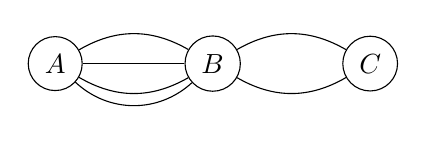
\begin{tikzpicture}
		\path (0,0)node[draw,circle](A){$A$};
		\path (2,0)node[draw,circle](B){$B$};
		\path (4,0)node[draw,circle](C){$C$};
		\draw (A)--(B);
		\draw(A)to[bend right](B) (A)to[bend left](B)(A)to[bend right=1.5cm](B)(B)to[bend right](C)(B)to[bend left](C);
	\end{tikzpicture}
\end{center}
\choice
{\True 8}
{12}
{4}
{6}
\loigiai{
Đi từ thành phố $A$ qua thành phố $B$ có $4$ cách.\\
Đi từ thành phố $B$ qua thành phố $C$ có $2$ cách.\\
Theo quy tắc nhân, có $4\cdot 2=8$ cách đi từ thành phố $A$ đến thành phố $C$ mà chỉ qua thành phố $B$ một lần.
}
\end{ex}
\begin{ex}%[0H4B1-4]%[Dự án Đề kiểm tra HKII NH22-23-TinDatTran]%[THPT Nguyễn Trường Tộ - Huế]
Tính góc giữa hai đường thẳng $\Delta\colon x-\sqrt{3} y+1=0$ và $\Delta'\colon x+\sqrt{3} y=0$?
\choice
{$120^{\circ}$}
{\True $60^{\circ}$}
{$90^{\circ}$}
{$30^{\circ}$}
\loigiai{
Vectơ pháp tuyến của $\Delta$ và $\Delta'$ là $\vec{n}_\Delta=(1;-\sqrt{3})$, $\vec{n}_{\Delta'}=(1;\sqrt{3})$.\\
Ta có
\[\cos(\Delta;\Delta')=\dfrac{|\vec{n}_{\Delta}\cdot \vec{n}_{\Delta'}|}{|\vec{n}_{\Delta}|
\cdot |\vec{n}_{\Delta'}|}=\dfrac{1}{2}\Rightarrow (\Delta;\Delta')=60^\circ.\]
}
\end{ex}
\begin{ex}%[0H4Y3-4]%[Dự án Đề kiểm tra HKII NH22-23-TinDatTran]%[THPT Nguyễn Trường Tộ - Huế]
Trong mặt phẳng $Oxy$, với $a, b, p>0$, phương trình chính tắc của một hypebol có dạng
\choice
{$y^2=2 p x$}
{\True $\dfrac{x^2}{a^2}-\dfrac{y^2}{b^2}=1$}
{$\dfrac{x^2}{a^2}+\dfrac{y^2}{b^2}=1$}
{$y^2=p x$}
\loigiai{
Trong mặt phẳng $Oxy$, với $a, b, p>0$, phương trình chính tắc của một hypebol có dạng $\dfrac{x^2}{a^2}-\dfrac{y^2}{b^2}=1$.
}
\end{ex}
\begin{ex}%[0X2B2-4]%[Dự án Đề kiểm tra HKII NH22-23-TinDatTran]%[THPT Nguyễn Trường Tộ - Huế]
Trong mặt phẳng cho tập hợp $P$ gồm 10 điểm phân biệt trong đó không có 3 điểm nào thẳng hàng. Số tam giác có 3 đỉnh đều thuộc $P$ là
\choice
{\True $\mathrm{C}_{10}^3$}
{$10^3$}
{$\mathrm{A}_{10}^3$}
{$\mathrm{A}_{10}^7$}
\loigiai{
Chọn 3 điểm từ tập hợp $P$ có $\mathrm{C}_{10}^3$ cách nên số tam giác có 3 đỉnh đều thuộc $P$ là $\mathrm{C}_{10}^3$.
}
\end{ex}
\begin{ex}%[0X2B1-2]%[Dự án Đề kiểm tra HKII NH22-23-TinDatTran]%[THPT Nguyễn Trường Tộ - Huế]
Một nhóm học sinh có 5 nam, 6 nữ. Hỏi có bao nhiêu cách chọn 1 học sinh nam và 1 học sinh nữ lên bảng làm bài tập?
\choice
{11}
{\True 30}
{6}
{5}
\loigiai{
Chọn 1 học sinh nam có 5 cách.\\
Chọn 1 học sinh nữ có 6 cách.\\
Theo quy tắc nhân, ta có $5\cdot 6=30$ cách chọn 1 học sinh nam và 1 học sinh nữ lên bảng làm bài tập.
}
\end{ex}
\begin{ex}%[0X2Y2-2]%[Dự án Đề kiểm tra HKII NH22-23-TinDatTran]%[THPT Nguyễn Trường Tộ - Huế]
Một hộp chứa 6 bi xanh và 4 bi đỏ. Có bao nhiêu cách lấy ngẫu nhiên 3 viên bi từ hộp bi?
\choice
{480}
{\True 120}
{720}
{80}
\loigiai{
Chọn $3$ viên bi từ hộp bi trên có $\mathrm{C}_{10}^3=120$ cách.
}
\end{ex}
\begin{ex}%[0H4B3-1]%[Dự án Đề kiểm tra HKII NH22-23-TinDatTran]%[THPT Nguyễn Trường Tộ - Huế]
Trong mặt phẳng $Oxy$, cho elip $(E)\colon \dfrac{x^2}{25}+\dfrac{y^2}{9}=1$. Khi đó, tiêu cự của elip bằng
\choice
{10}
{6}
{\True 8}
{4}
\loigiai{
Ta có $(E)\colon \dfrac{x^2}{25}+\dfrac{y^2}{9}=1\Rightarrow \heva{&a=5\\&b=3.}$\\
Tiêu cự của elip là $2c=\sqrt{a^2-b^2}=2\sqrt{5^2-3^2}=2\cdot4=8$.
}
\end{ex}
\begin{ex}%[0H4K1-3]%[Dự án Đề kiểm tra HKII NH22-23-TinDatTran]%[THPT Nguyễn Trường Tộ - Huế]
Cho hai đường thẳng: $2 x-y-1=0$ và $x+2 y+2=0$. Khi nói về vị trí tương đối của chúng, khẳng định nào đúng?
\choice
{Cắt nhau nhưng không vuông góc}
{\True Vuông góc}
{Song song}
{Trùng nhau}
\loigiai{
Hai đường thẳng đã cho có hai vectơ pháp tuyến lần lượt là $\vec{n}_1=(2;-1)$, $\vec{n}_2=(1;2)$.\\
Vì $\vec{n}_1\cdot \vec{n}_2=2\cdot 1+(-1)\cdot 2=0$ nên hai đường thẳng đã cho vuông góc với nhau.
}
\end{ex}
\begin{ex}%[0X2B2-2]%[Dự án Đề kiểm tra HKII NH22-23-TinDatTran]%[THPT Nguyễn Trường Tộ - Huế]
Lớp 10B có 25 đoàn viên trong đó 10 nam và 15 nữ. Chọn ngẫu nhiên 3 đoàn viên trong lớp để tham dự hội trại ngày 26 tháng 3. Tính xác suất để 3 đoàn viên được chọn có 2 nam và 1 nữ?
\choice
{$\dfrac{9}{92}$}
{$\dfrac{3}{115}$}
{$\dfrac{7}{920}$}
{\True $\dfrac{27}{92}$}
\loigiai{
Số cách để chọn ngẫu nhiên 3 đoàn viên tham dự hội trại là $\mathrm{C}_{25}^3\Rightarrow n(\Omega)=\mathrm{C}_{25}^3$.
Gọi $A$ là biến cố ``Chọn 3 đoàn viên tham dự trong đó có 2 nam và 1 nữ''.
\begin{itemize}
\item Chọn $2$ đoàn viên nam có $C_{10}^2$ cách.
\item Chọn $1$ đoàn viên nữ có $C_{15}^1$ cách.
\end{itemize}
Theo quy tắc nhân, ta có $n(A)=\mathrm{C}_{10}^2\cdot \mathrm{C}_{15}^1$.\\
Vậy xác suất cần tìm là $P(A)=\dfrac{n(A)}{n(\Omega)}\dfrac{\mathrm{C}_{10}^2\cdot \mathrm{C}_{15}^1}{\mathrm{C}_{25}^3}=\dfrac{27}{92}$.
}
\end{ex}
\begin{ex}%[0D3B2-3]%[Dự án Đề kiểm tra HKII NH22-23-TinDatTran]%[THPT Nguyễn Trường Tộ - Huế]
Cho hàm số $y=x^2-3 x+2$. Phương trình trục đối xứng của đồ thị hàm số là
\choice
{\True $x=\dfrac{3}{2}$}
{$y=\dfrac{3}{2}$}
{$y=-\dfrac{3}{2}$}
{$x=-\dfrac{3}{2}$}
\loigiai{
Trục đối xứng của đồ thị hàm số trên là $x=\dfrac{-b}{2a}=\dfrac{3}{2}$.
}
\end{ex}
\begin{ex}%[0X3Y2-6]%[Dự án Đề kiểm tra HKII NH22-23-TinDatTran]%[THPT Nguyễn Trường Tộ - Huế]
Từ các số $1,2,3,4,6,7,8,9$ lấy ngẫu nhiên một số. Xác suất để lấy được số chẵn bằng:
\choice
{$\dfrac{1}{6}$}
{$\dfrac{1}{4}$}
{$\dfrac{2}{3}$}
{\True $\dfrac{1}{2}$}
\loigiai{
Ta có $n(\Omega)=8$.\\
Gọi $A$ là biến cố ''Lấy được một số chẵn từ các số $1,2,3,4,6,7,8,9$''. Ta có $n(A)=4$
Suy ra xác suất cần tìm là $P(A)=\dfrac{n(A)}{n(\Omega)}\dfrac{4}{8}=\dfrac{1}{2}$.
}
\end{ex}
\begin{ex}%[0X2B2-3]%[Dự án Đề kiểm tra HKII NH22-23-TinDatTran]%[THPT Nguyễn Trường Tộ - Huế]
Cho tập $X$ có 9 phần tử. Tìm số tập con có 5 phần tử của tập $X$.
\choice
{$216$}
{\True $126$}
{$15120$}
{$120$}
\loigiai{
Số tập con có $5$ phần tử của tập $X$ là $C_9^5=126$.
}
\end{ex}
\begin{ex}%[0H4B1-5]%[Dự án Đề kiểm tra HKII NH22-23-TinDatTran]%[THPT Nguyễn Trường Tộ - Huế]
Tính khoảng cách từ điểm $M(2 ; 1)$ đến đường thẳng $3 x-4 y+1=0$.
\choice
{\True $\dfrac{3}{5}$}
{$\dfrac{2}{5}$}
{$\dfrac{8}{5}$}
{$\dfrac{9}{5}$}
\loigiai{
Khoảng cách cần tìm là $d=\dfrac{3\cdot 2-4\cdot 1+1}{\sqrt{3^2+(-4)^2}}=\dfrac{3}{5}$.
}
\end{ex}
\begin{ex}%[0D3Y1-2]%[Dự án Đề kiểm tra HKII NH22-23-TinDatTran]%[THPT Nguyễn Trường Tộ - Huế]
Tập xác định của hàm số $y=\dfrac{3}{x-5}$ là
\choice
{$D=(5 ;+\infty)$}
{$D= \mathbb{R}$}
{\True $D= \mathbb{R} \backslash\{5\}$}
{$D= \mathbb{R} \backslash\{-5\}$}
\loigiai{
Điều kiện xác định $x-5\neq 0\Leftrightarrow x\neq 5$.\\
Tập xác định của hàm số $y=\dfrac{3}{x-5}$ là $D= \mathbb{R} \backslash\{5\}$.
}
\end{ex}
\begin{ex}%[0X2Y2-1]%[Dự án Đề kiểm tra HKII NH22-23-TinDatTran]%[THPT Nguyễn Trường Tộ - Huế]
Có bao nhiêu cách xếp 7 học sinh thành một hàng dọc?
\choice
{$49$}
{\True $5040$}
{$7$}
{$1$}
\loigiai{
Số cách xếp $7$ học sinh thành một hàng dọc là $7!=5040$ cách.
}
\end{ex}
\begin{ex}%[0X3B2-4]%[Dự án Đề kiểm tra HKII NH22-23-TinDatTran]%[THPT Nguyễn Trường Tộ - Huế]
Trong một hộp có 5 bi xanh và 4 bi đỏ. Lấy ngẫu nhiên ra 2 viên bi. Xác suất để 2 viên bi lấy ra có cùng màu là
\choice
{\True $\dfrac{4}{9}$}
{$\dfrac{3}{18}$}
{$\dfrac{5}{18}$}
{$\dfrac{2}{9}$}
\loigiai{
Ta có $n(\Omega)=\mathrm{C}_9^2$.\\
Gọi $A$ là biến cố ``Lấy được 2 viên bi cùng màu''. Ta có hai trường hợp
\begin{itemize}
\item Lấy được hai viên bi màu xanh có $\mathrm{C}_5^2$ cách.
\item Lấy được hai viên bi màu đỏ có $\mathrm{C}_4^2$ cách.
\end{itemize}
Suy ra $n(A)=\mathrm{C}_5^2+\mathrm{C}_4^2$.\\
Xác suất để 2 viên bi lấy ra có cùng màu là
\[P(A)=\dfrac{n(A)}{n(\Omega)}=\dfrac{\mathrm{C}_5^2+ \mathrm{C}_4^2}{\mathrm{C}_9^2}=\dfrac{4}{9}.\]
}
\end{ex}


\Closesolutionfile{ans}
\begin{center}
	\textbf{ĐÁP ÁN}
	\inputansbox{10}{ans/ans}	
\end{center}
\begin{center}
	\textbf{PHẦN 2 - TỰ LUẬN}
\end{center}
\begin{bt}%[0H4K2-2]%[Dự án Đề kiểm tra HKII NH22-23-TinDatTran]%[THPT Nguyễn Trường Tộ - Huế]
Trong mặt phẳng tọa độ $O x y$, cho tam giác $A B C$ có $A(2 ; 0), B(0 ; 3), C(-3 ; 1)$.
\begin{enumerate}
\item Viết phương trình tổng quát của thẳng $d$ đi qua $B$ và song song với $A C$.
\item Viết phương trình đường tròn ngoại tiếp tam giác $A B C$.
\end{enumerate}
\loigiai{
\begin{enumerate}
\item Ta có $\overrightarrow{A C}=(-5 ; 1)$.\\
Vì đường thẳng $d$ song song với $A C$ nên $d$ nhận $\overrightarrow{A C}$ là vectơ chỉ phương.\\
Suy ra vectơ pháp tuyến của $d$ là $\vec{n}=(1 ; 5)$.\\
Phương trình đường thẳng $d$ qua $B(0 ; 3)$ có vectơ pháp tuyến $\vec{n}=(1 ; 5)$ là 
\[1(x-0)+5(y-3)=0 \Leftrightarrow x+5 y-15=0.\]
\item Gọi phương trình đường tròn cần tìm dạng: $x^2+y^2-2 a x-2 b y+c=0\left(a^2+b^2-c>0\right)$.
Đường tròn đi qua 3 điểm $A(2 ; 0), B(0 ; 3), C(-3 ; 1)$ nên ta có:
\[\heva{&-4 a+c=-4 \\&-6 b+c=-9 \\&6 a-2 b+c=-10}\Leftrightarrow\heva{&a=\dfrac{-1}{2} \\&b=\dfrac{1}{2} \\&c=-6.}\]
Vậy phương trình đường tròn ngoại tiếp tam giác $A B C$ là 
\[x^2+y^2+x-y-6=0.\]
\end{enumerate}
}
\end{bt}
\begin{bt}%[0X2K2-4]%[Dự án Đề kiểm tra HKII NH22-23-TinDatTran]%[THPT Nguyễn Trường Tộ - Huế]
\begin{enumerate}
\item Khai triển nhị thức sau $(2 x-3)^4$.
\item Tìm số đỉnh của một đa giác lồi, biết đa giác đó có 54 đường chéo.
\end{enumerate}
\loigiai{
\begin{enumerate}
\item 
Ta có
\begin{eqnarray*}
	(2 x-3)^4&=&\mathrm{C}_4^0(2 x)^4+\mathrm{C}_4^1(2 x)^3(-3)+\mathrm{C}_4^2(2 x)^2(-3)^2+\mathrm{C}_4^3 2 x (-3)^3+\mathrm{C}_4^4(-3)^4 \\ 
	& =&16 x^4-96 x^3+216 x^2-216 x+81.
\end{eqnarray*}
\item Giả sử đa giác có $n$ đỉnh $(n \geq 3, n \in \mathbb{N})$.\\
Đa giác đó có 54 đường chéo nên ta có: 
\[
C_n^2-n=54\Leftrightarrow n^2-3 n-108=0 \Leftrightarrow\hoac{&n=12~(\text{thỏa}) \\&n=-9~(\text{không thỏa mãn}).}
\]
Vậy đa giác có 12 đỉnh.
\end{enumerate}
}
\end{bt}
\begin{bt}%[0X3G2-6]%[Dự án Đề kiểm tra HKII NH22-23-TinDatTran]%[THPT Nguyễn Trường Tộ - Huế]
Từ tập hợp các số tự nhiên có sáu chữ số đôi một khác nhau được lập từ tập $M=\{1 ; 2 ; 3 ; 4 ; 5 ; 6\}$, chọn ngẫu nhiên một số. Tính xác suất để số được chọn có tổng ba chữ số đầu nhỏ hơn tổng ba chữ số cuối một đơn vị.
\loigiai{
Số số tự nhiên có sáu chữ số khác nhau được lập từ tập M là $6 !=720$ số $\Rightarrow n(\Omega)=720$.\\
Gọi số tự nhiên có sáu chữ số khác nhau có tổng ba chữ số đầu bé hơn tổng ba chữ số cuối một đơn vị là $\overline{a b c d e f}$.\\\
Ta có $\heva{&a+b+c+d+e+f=21 \\ &(d+e+f)-(a+b+c)=1} \Leftrightarrow\heva{&a+b+c=10 \\ &d+e+f=11.}$\\
Nên ta có các trường hợp sau:
\begin{itemize}
\item \textbf{Trường hợp 1}: $a, b, c \in\{1 ; 3 ; 6\}$ và $d, e, f \in\{2 ; 4 ; 5\}$. Khi đó có $3!\cdot 3!=36$ số.
\item \textbf{Trường hợp 2}: $a, b, c \in\{1 ; 4 ; 5\}$ và $d, e, f \in\{2 ; 3 ; 6\}$. Khi đó có $3! \cdot 3!=36$ số.
\item \textbf{Trường hợp 3}: $a, b, c \in\{2 ; 3 ; 5\}$ và $d, e, f \in\{1 ; 4 ; 6\}$. Khi đó có $3! \cdot 3!=36$ số.
\end{itemize}
Nên có tất cả $36+36+36=108$ số.\\
Gọi $A$ là biến cố: ``Số được chọn có tổng ba chữ số đầu nhỏ hơn tổng ba chữ số cuối một đơn vị''.\\
$\Rightarrow n(A)=108$.\\
Vậy $P(A)=\dfrac{n(A)}{n(\Omega)}=\dfrac{108}{720}=\dfrac{3}{20}$.
}
\end{bt}